
%% bare_conf.tex
%% V1.4b
%% 2015/08/26
%% by Michael Shell
%% See:
%% http://www.michaelshell.org/
%% for current contact information.
%%
%% This is a skeleton file demonstrating the use of IEEEtran.cls
%% (requires IEEEtran.cls version 1.8b or later) with an IEEE
%% conference paper.
%%
%% Support sites:
%% http://www.michaelshell.org/tex/ieeetran/
%% http://www.ctan.org/pkg/ieeetran
%% and
%% http://www.ieee.org/

%%*************************************************************************
%% Legal Notice:
%% This code is offered as-is without any warranty either expressed or
%% implied; without even the implied warranty of MERCHANTABILITY or
%% FITNESS FOR A PARTICULAR PURPOSE! 
%% User assumes all risk.
%% In no event shall the IEEE or any contributor to this code be liable for
%% any damages or losses, including, but not limited to, incidental,
%% consequential, or any other damages, resulting from the use or misuse
%% of any information contained here.
%%
%% All comments are the opinions of their respective authors and are not
%% necessarily endorsed by the IEEE.
%%
%% This work is distributed under the LaTeX Project Public License (LPPL)
%% ( http://www.latex-project.org/ ) version 1.3, and may be freely used,
%% distributed and modified. A copy of the LPPL, version 1.3, is included
%% in the base LaTeX documentation of all distributions of LaTeX released
%% 2003/12/01 or later.
%% Retain all contribution notices and credits.
%% ** Modified files should be clearly indicated as such, including  **
%% ** renaming them and changing author support contact information. **
%%*************************************************************************


% *** Authors should verify (and, if needed, correct) their LaTeX system  ***
% *** with the testflow diagnostic prior to trusting their LaTeX platform ***
% *** with production work. The IEEE's font choices and paper sizes can   ***
% *** trigger bugs that do not appear when using other class files.       ***                          ***
% The testflow support page is at:
% http://www.michaelshell.org/tex/testflow/



\documentclass[conference]{IEEEtran}
% Some Computer Society conferences also require the compsoc mode option,
% but others use the standard conference format.
%
% If IEEEtran.cls has not been installed into the LaTeX system files,
% manually specify the path to it like:
% \documentclass[conference]{../sty/IEEEtran}





% Some very useful LaTeX packages include:
% (uncomment the ones you want to load)


% *** MISC UTILITY PACKAGES ***
%
%\usepackage{ifpdf}
% Heiko Oberdiek's ifpdf.sty is very useful if you need conditional
% compilation based on whether the output is pdf or dvi.
% usage:
% \ifpdf
%   % pdf code
% \else
%   % dvi code
% \fi
% The latest version of ifpdf.sty can be obtained from:
% http://www.ctan.org/pkg/ifpdf
% Also, note that IEEEtran.cls V1.7 and later provides a builtin
% \ifCLASSINFOpdf conditional that works the same way.
% When switching from latex to pdflatex and vice-versa, the compiler may
% have to be run twice to clear warning/error messages.

% *** CITATION PACKAGES ***
%
\usepackage{cite}
% cite.sty was written by Donald Arseneau
% V1.6 and later of IEEEtran pre-defines the format of the cite.sty package
% \cite{} output to follow that of the IEEE. Loading the cite package will
% result in citation numbers being automatically sorted and properly
% "compressed/ranged". e.g., [1], [9], [2], [7], [5], [6] without using
% cite.sty will become [1], [2], [5]--[7], [9] using cite.sty. cite.sty's
% \cite will automatically add leading space, if needed. Use cite.sty's
% noadjust option (cite.sty V3.8 and later) if you want to turn this off
% such as if a citation ever needs to be enclosed in parenthesis.
% cite.sty is already installed on most LaTeX systems. Be sure and use
% version 5.0 (2009-03-20) and later if using hyperref.sty.
% The latest version can be obtained at:
% http://www.ctan.org/pkg/cite
% The documentation is contained in the cite.sty file itself.








% *** MATH PACKAGES ***
%
\usepackage{amsmath}
% A popular package from the American Mathematical Society that provides
% many useful and powerful commands for dealing with mathematics.
%
% Note that the amsmath package sets \interdisplaylinepenalty to 10000
% thus preventing page breaks from occurring within multiline equations. Use:
%\interdisplaylinepenalty=2500
% after loading amsmath to restore such page breaks as IEEEtran.cls normally
% does. amsmath.sty is already installed on most LaTeX systems. The latest
% version and documentation can be obtained at:
% http://www.ctan.org/pkg/amsmath





% *** SPECIALIZED LIST PACKAGES ***
%
%\usepackage{algorithmic}
% algorithmic.sty was written by Peter Williams and Rogerio Brito.
% This package provides an algorithmic environment fo describing algorithms.
% You can use the algorithmic environment in-text or within a figure
% environment to provide for a floating algorithm. Do NOT use the algorithm
% floating environment provided by algorithm.sty (by the same authors) or
% algorithm2e.sty (by Christophe Fiorio) as the IEEE does not use dedicated
% algorithm float types and packages that provide these will not provide
% correct IEEE style captions. The latest version and documentation of
% algorithmic.sty can be obtained at:
% http://www.ctan.org/pkg/algorithms
% Also of interest may be the (relatively newer and more customizable)
% algorithmicx.sty package by Szasz Janos:
% http://www.ctan.org/pkg/algorithmicx




% *** ALIGNMENT PACKAGES ***
%
%\usepackage{array}
% Frank Mittelbach's and David Carlisle's array.sty patches and improves
% the standard LaTeX2e array and tabular environments to provide better
% appearance and additional user controls. As the default LaTeX2e table
% generation code is lacking to the point of almost being broken with
% respect to the quality of the end results, all users are strongly
% advised to use an enhanced (at the very least that provided by array.sty)
% set of table tools. array.sty is already installed on most systems. The
% latest version and documentation can be obtained at:
% http://www.ctan.org/pkg/array


% IEEEtran contains the IEEEeqnarray family of commands that can be used to
% generate multiline equations as well as matrices, tables, etc., of high
% quality.




% *** SUBFIGURE PACKAGES ***
%\ifCLASSOPTIONcompsoc
%  \usepackage[caption=false,font=normalsize,labelfont=sf,textfont=sf]{subfig}
%\else
%  \usepackage[caption=false,font=footnotesize]{subfig}
%\fi
% subfig.sty, written by Steven Douglas Cochran, is the modern replacement
% for subfigure.sty, the latter of which is no longer maintained and is
% incompatible with some LaTeX packages including fixltx2e. However,
% subfig.sty requires and automatically loads Axel Sommerfeldt's caption.sty
% which will override IEEEtran.cls' handling of captions and this will result
% in non-IEEE style figure/table captions. To prevent this problem, be sure
% and invoke subfig.sty's "caption=false" package option (available since
% subfig.sty version 1.3, 2005/06/28) as this is will preserve IEEEtran.cls
% handling of captions.
% Note that the Computer Society format requires a larger sans serif font
% than the serif footnote size font used in traditional IEEE formatting
% and thus the need to invoke different subfig.sty package options depending
% on whether compsoc mode has been enabled.
%
% The latest version and documentation of subfig.sty can be obtained at:
% http://www.ctan.org/pkg/subfig




% *** FLOAT PACKAGES ***
%
%\usepackage{fixltx2e}
% fixltx2e, the successor to the earlier fix2col.sty, was written by
% Frank Mittelbach and David Carlisle. This package corrects a few problems
% in the LaTeX2e kernel, the most notable of which is that in current
% LaTeX2e releases, the ordering of single and double column floats is not
% guaranteed to be preserved. Thus, an unpatched LaTeX2e can allow a
% single column figure to be placed prior to an earlier double column
% figure.
% Be aware that LaTeX2e kernels dated 2015 and later have fixltx2e.sty's
% corrections already built into the system in which case a warning will
% be issued if an attempt is made to load fixltx2e.sty as it is no longer
% needed.
% The latest version and documentation can be found at:
% http://www.ctan.org/pkg/fixltx2e


%\usepackage{stfloats}
% stfloats.sty was written by Sigitas Tolusis. This package gives LaTeX2e
% the ability to do double column floats at the bottom of the page as well
% as the top. (e.g., "\begin{figure*}[!b]" is not normally possible in
% LaTeX2e). It also provides a command:
%\fnbelowfloat
% to enable the placement of footnotes below bottom floats (the standard
% LaTeX2e kernel puts them above bottom floats). This is an invasive package
% which rewrites many portions of the LaTeX2e float routines. It may not work
% with other packages that modify the LaTeX2e float routines. The latest
% version and documentation can be obtained at:
% http://www.ctan.org/pkg/stfloats
% Do not use the stfloats baselinefloat ability as the IEEE does not allow
% \baselineskip to stretch. Authors submitting work to the IEEE should note
% that the IEEE rarely uses double column equations and that authors should try
% to avoid such use. Do not be tempted to use the cuted.sty or midfloat.sty
% packages (also by Sigitas Tolusis) as the IEEE does not format its papers in
% such ways.
% Do not attempt to use stfloats with fixltx2e as they are incompatible.
% Instead, use Morten Hogholm'a dblfloatfix which combines the features
% of both fixltx2e and stfloats:
%
% \usepackage{dblfloatfix}
% The latest version can be found at:
% http://www.ctan.org/pkg/dblfloatfix

\usepackage{graphicx}
\usepackage{epstopdf}

% *** PDF, URL AND HYPERLINK PACKAGES ***
%
\usepackage{url}
% url.sty was written by Donald Arseneau. It provides better support for
% handling and breaking URLs. url.sty is already installed on most LaTeX
% systems. The latest version and documentation can be obtained at:
% http://www.ctan.org/pkg/url
% Basically, \url{my_url_here}.




% *** Do not adjust lengths that control margins, column widths, etc. ***
% *** Do not use packages that alter fonts (such as pslatex).         ***
% There should be no need to do such things with IEEEtran.cls V1.6 and later.
% (Unless specifically asked to do so by the journal or conference you plan
% to submit to, of course. )


% correct bad hyphenation here
\hyphenation{op-tical net-works semi-conduc-tor}


\begin{document}
%
% paper title
% Titles are generally capitalized except for words such as a, an, and, as,
% at, but, by, for, in, nor, of, on, or, the, to and up, which are usually
% not capitalized unless they are the first or last word of the title.
% Linebreaks \\ can be used within to get better formatting as desired.
% Do not put math or special symbols in the title.
\title{Security of Distribution Mechanisms for Linux and BSD Operating Systems}


% author names and affiliations
% use a multiple column layout for up to three different
% affiliations
\author{\IEEEauthorblockN{Gabriel Ewing}
\IEEEauthorblockA{Department of Electrical Engineering and\\Computer Science\\
Case Western Reserve University\\
Cleveland, Ohio}
\and
\IEEEauthorblockN{Kevin Nash}
\IEEEauthorblockA{Department of Electrical Engineering and\\Computer Science\\
Case Western Reserve University\\
Cleveland, Ohio}}

% conference papers do not typically use \thanks and this command
% is locked out in conference mode. If really needed, such as for
% the acknowledgment of grants, issue a \IEEEoverridecommandlockouts
% after \documentclass

% for over three affiliations, or if they all won't fit within the width
% of the page, use this alternative format:
% 
%\author{\IEEEauthorblockN{Michael Shell\IEEEauthorrefmark{1},
%Homer Simpson\IEEEauthorrefmark{2},
%James Kirk\IEEEauthorrefmark{3}, 
%Montgomery Scott\IEEEauthorrefmark{3} and
%Eldon Tyrell\IEEEauthorrefmark{4}}
%\IEEEauthorblockA{\IEEEauthorrefmark{1}School of Electrical and Computer Engineering\\
%Georgia Institute of Technology,
%Atlanta, Georgia 30332--0250\\ Email: see http://www.michaelshell.org/contact.html}
%\IEEEauthorblockA{\IEEEauthorrefmark{2}Twentieth Century Fox, Springfield, USA\\
%Email: homer@thesimpsons.com}
%\IEEEauthorblockA{\IEEEauthorrefmark{3}Starfleet Academy, San Francisco, California 96678-2391\\
%Telephone: (800) 555--1212, Fax: (888) 555--1212}
%\IEEEauthorblockA{\IEEEauthorrefmark{4}Tyrell Inc., 123 Replicant Street, Los Angeles, California 90210--4321}}




% use for special paper notices
%\IEEEspecialpapernotice{(Invited Paper)}




% make the title area
\maketitle

% As a general rule, do not put math, special symbols or citations
% in the abstract
\begin{abstract}
    We investigate the issue of the security of distribution of images of
    open-source operating systems. We review the stages in a common
    distribution process, possible attacks on the process, and 
    practices of individual distributions. We use work in the literature
    on cryptographic algorithms to identify algorithms that should not be
    used in this context. We offer guidelines for how
    distributions can secure their distribution processes and how
    consumers can best insulate themselves from the associated risks.
\end{abstract}

% no keywords




% For peer review papers, you can put extra information on the cover
% page as needed:
% \ifCLASSOPTIONpeerreview
% \begin{center} \bfseries EDICS Category: 3-BBND \end{center}
% \fi
%
% For peerreview papers, this IEEEtran command inserts a page break and
% creates the second title. It will be ignored for other modes.
\IEEEpeerreviewmaketitle\


\section{Introduction}

An operating system is a piece of software that manages computer hardware resources
and provides a variety of services for computer programs.
The central core of an operating system, its kernel, is the first layer
above hardware itself. Due to of the depth of their functionality,
compromised operating systems can potentially yield a great deal more power
to an attacker than application software.\\
\indent Operating systems can be compromised by malicious computer software,
such as rootkits, in the course of normal operation. However, attacks can sometimes
be launched more easily against the distribution process itself. This can be done in such a way
that users unknowingly install a modified version of the expected operating
system. If successful, attacks that result in the distribution of a compromised
operating system can be both difficult to detect and
powerful.\\
\indent The open-source software model possesses a somewhat different attack surface that its closed- or shared-source counterparts.
Open-source operating systems often have much smaller core development teams
than popular commercial systems such as Windows and OS X. Open-source operating systems are rarely distributed using
physical media, which is the primary distribution mechanism for Windows.
The commercial interfaces that are requisite for online distribution of proprietary
software also have advantages and disadvantages in security that
are different from the security considerations that open-source distributors must account for.\\
\indent In the course of research for this paper, we looked at the top ten Linux distributions
on DistroWatch~\cite{DistroWatch}, plus Slackware Linux, Gentoo Linux, FreeBSD, and OpenBSD.\@
We noted the default installation choices that these distributions offer to users, recent
news involving them, and various miscellaneous pieces of information. In this paper, we present
and discuss our most interesting findings.

\subsection{Effects of Compromised Operating System}

Allowing an attacker to write an arbitrary operating system that is subsequently
installed on a server or personal computer offers an extraordinary level of
invasion of privacy and system access. Every action that a user takes on a
computer goes through the operating system. It would be trivial to write a logger
for all network traffic on a computer and periodically send it to the attacker. If
the compromised system is a web server, all information stored in the database would
be freely available unless encrypted before it reached the server. A laptop with a
built-in or external camera could broadcast all visible activities to an attacker.
A keylogger could log credit cards and passwords and transmit them periodically.
Perhaps the most likely action by an attacker would be to use the malicious
operating system as part of a botnet, sending spam emails or carrying out denial-
of-service attacks. While these may not directly impact the user, they have a
negative effect on the global state of security. Great care should be taken to avoid
the installation of compromised operating systems.

\subsection{Conventions}

In this paper, we frequently refer to installation images. These are usually~.iso
files that can be burned to some physical media and installed on a system. Another
way to install an open-source operating system is to build the system from source
code. Building from source offers the advantage of being able to read code before
building an image from it, and can be safer than directly installing an image.
Modern operating systems, though, contain millions of lines of code and it is
difficult or impossible for any individual or group to conduct a meaningful and
comprehensive code review before building from source. This means that many issues
affecting binary images also affect source code releases. Unless otherwise specified,
when we refer to installation images, we mean that to include source releases.\\
\indent We investigated operating systems from the Linux and BSD families. We refer to any
member of these that is a complete operating system that publishes their own releases
as a ``distribution'', even though this more commonly is used for Linux releases
than BSD.\\
\indent Similarly, we use the phrase ``open source'' to refer to any piece of
software whose source code is publicly available and may be installed at no cost.
This includes software whose creators prefer the term ``free software''.

\section{Operating System Distribution}

The specific process by which a new version of an operating system
travels from developer to end user differs between development teams.
Operating system developers establish their own schedule
standardizations, though the time between starting the release process
and the anticipated release typically takes no more than 90 days.
Some teams may implement some steps less formally than others do,
though the general procedures are common enough between projects they can be
summarized by a few key steps.

\subsection{System Changes}

In an operating system's natural lifecycle, users tend to discover that
the system exhibits certain unexpected behaviors.
These bugs are reported, tracked, and hopefully fixed in code so that
users will not experience them in future versions of the operating system.
Users might request that entirely new features be added
or that existing, intentional behaviors be modified.
Even without user input, changes to the system inevitably
originate from within the development team; design paradigms change
and the best practices in security as well as trends in operating system design
are ever-evolving.\\
\indent No matter the cause, an operating system's codebase can change
frequently. After enough changes are made to warrant a new release,
or at certain milestones in a predetermined development schedule,
developers stop making new changes in preparation for a code review.
Then most developers of different operating systems will ``freeze''
or ``lock'' the code so that no more changes can be made.
Before the code freeze occurs, developers finish integrating their changes
and merge the development branch into a stable, or production, branch.
Of course, the naming of branches varies between projects.
Once the code is frozen, the interested public and, in almost all cases,
an internal body performs a code review.

\subsection{Code Review}
Ideally, code is reviewed on a rolling basis
throughout the release cycle so that reviewers have time to also deal with any new bugs
that come up. 
In general, the code is reviewed for proper practice and adherence to in-house standards.
Code reviewers must be very careful, because detecting subtly inserted malicious
code can be a hard task. Many distributions are forced to rely on trust in the
code authors to not make deliberate mistakes, and the reviews are only deep
enough to catch unintentional bugs.

\subsection{Testing}
A beta image is built and distributed to testers.
New features are tested for proper functionality, and bug fixes are tested for robustness.
As necessary minor changes are made, such as those to update documentation,
fix remaining bugs, and address any discovered security issues,
additional beta images will be released for testing~\cite{freebsdrelease}.
Software development processes and schedules are well-studied and too complex to cover well in this
paper.

\subsection{Release Building}
Once the beta images are proven to meet quality standards,
a branch for the new version is created.
The most successful beta images will be included on the branch
as ``release candidates'' a term for beta versions of software
that have the potential to be a finished product.
The release candidates will undergo further stability testing.
Eventually, a release candidate (not necessarily the most recent) will
be selected as the final, stable version~\cite{freebsdrelease}.

\begin{figure}[h!]
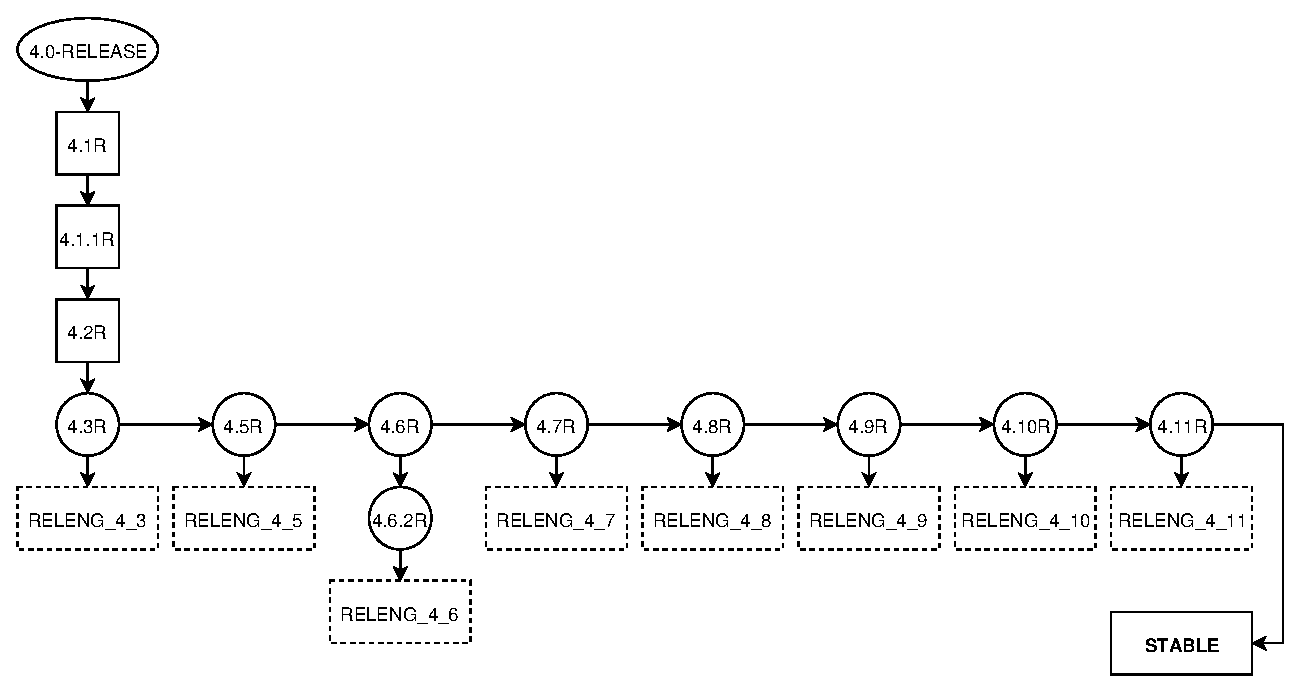
\includegraphics[width=\linewidth]{./images/FreeBSD_4.eps}
\caption{FreeBSD's RELENG\_4 (4.x STABLE Branch)}
\label{FreeBSD_4}
\end{figure}

\subsection{Pre-Distribution}
Once the stable release image has been slated for distribution,
the mirror sites must be updated to serve this new image.
Release engineers will coordinate with the administrators of their mirror
sites to ensure that the sites have download access to the new image and
that the site is aware of the staged release.
Because each mirror site may be managed by an independent administrator,
it can take multiple days for all FTP and HTTP sites
to reflect the new software.
The process of coordinating with the mirror sites is a crucial final step
on the release team's end, so it is begun several days before
the public release day.
A file enumerating the hashes for each architecture is distributed 
alongside the installation images themselves.
This file is made available via the mirror site, or the hashes are displayed
on the web page beside download hyperlinks, or both.
Once release day arrives and a given mirror site has
the new operating system, it will announce the public availability
of the new software~\cite{freebsdftp}.

\subsection{Image Mirroring}
Administrators of mirror sites have their own tasks
in ensuring a successful software release.
They maintain at least one local copy of the operating system,
ensuring that it is kept up-to-date, that its synchronization
is error-free, and that their hosting resources are healthy
and fully utilized by the public~\cite{freebsdmirror}.

\subsubsection{Mirror Qualifications}
The qualifications and requirements for official mirrors of operating systems
vary by the system in question, and different areas of distribution
differ in their own inherent requirements.
For example, an FTP site often represents the largest amount of data
that needs to be mirrored; it can contain a live file system,
the images of the installation distribution, and branches
or snapshots of checked-out source trees.
The amount of required space is also multiplied
by the number of operating system versions and architectures~\cite{ubuntumirror}~\cite{freebsdrequirements}.\\
\indent All operating system archives demand a certain minimum
amount of disk space. Keeping the archives uncorrupted and on-disk is
one of the primary requirements of a mirror.
The full distribution can have a size anywhere from 500 gigabytes to
multiple terabytes, depending on the size of operating system,
the number of snapshots and releases to be offered, and the number of
architectures supported. For example, at the time of this writing,
the Ubuntu archive uses 912GB of disk space and FreeBSD uses 1.4TB for its FTP distribution~\cite{ubuntumirror}~\cite{freebsdrequirements}.\\
\indent There are a number of system requirements that depend on
the expected number of clients. Since official mirrors are designed
to handle large volumes of traffic, official mirrors can be required to
meet hard standards above the inherent needs of a server.
These standards can include minimum CPU speeds, amounts of random access
memory, and even certain disk configurations such as RAID~\cite{ubuntumirror}~\cite{freebsdrequirements}.\\
\indent Finally, operating system authorities might have policies
unrelated to hardware, such as requirements about frequency of synchronization and refusal of upload connections. The previous
two requirements examples of distributions attempting to set some security standards for their mirrors.
As an example of a requirement not necessarily directly related to security, FreeBSD requires
that mirrors update once per day, at a minimum. Ubuntu requires that its country-level mirrors
update every six hours for archives or every four hours for active releases~\cite{ubuntumirror}~\cite{freebsdrequirements}.

\subsubsection{Fetching Release}
Offering up-to-date versions of an operating system across several
mirrors presents the challenge of ensuring all mirrors host the same content.
To accomplish this reliably, servers commonly use specialized software that
synchronizes files between two different systems.\
rsync is a widely-used utility that functions as both a file synchronization
and file transfer program. It minimizes network usage by implementing a
type of delta encoding. With this utility, the operators of mirror
servers operators can fetch a new installation image upon release and periodically
check for differences (deltas) between an image on the master server and
the local copy~\cite{ubuntursync}.\\
\indent By default rsync compares metadata, specifically the size and modification time, of files. This comparison can be done very quickly,
but it is not comprehensive and will not synchronize modifications that
do not change this metadata. An alternative behavior can be invoked,
however; calling a check with the option \texttt{--checksum} will split
its file into chunks and compute a set of two checksums for each chunk.
The first is a speedy rolling hash and the second is a more traditional
MD5 hash. These sums are then passed to the master server,
which will send the chunks whose rolling hashes differ from
those computed by the calling server. If the rolling hashes match,
the master server will compute the slower MD5 hash and compare it against
the MD5 hash that it received from the calling server. In this way
only parts of a file that have been modified are sent~\cite{ubuntuzsync}~\cite{sambarsync}.\\
\indent The rolling checksum has a length of 32 bits, and MD5 uses a
length of 128 bits; combining the two yields an entropy of
\begin{align*}
2^{32+128}=2^{160}
\end{align*}
and therefore it is very unlikely that rsync will fail to detect 
a modification~\cite{rsyncmath}. It is worth mentioning that the purpose of rsync's
\texttt{--checksum} option is not to ensure cryptographic security but
rather to ensure that modifications to master files---imagine those on a
frequently changing beta image---are noticed and synchronized without
needing to fetch the entire release~\cite{ubuntuzsync}.

\subsection{Distribution Methods}

Linux and BSD distros are usually offered over a variety of protocols,
each with separate advantages and disadvantages. The File Transfer Protocol (FTP) and 
the HyperText Transfer Protocol (HTTP) are very
similar. In the present day, the efficiencies of both are intimately
tied to TCP.\@ The analysis of and means by which BitTorrent works are rather different. Transferring physical media is incomparable to any of
the other protocols from a network analyst's perspective.

\subsubsection{FTP and HTTP}
FTP is older than HTTP and features a few
inefficiencies that HTTP addresses. First, FTP spends three round trips
as overhead in getting the first file and two round trips
as overhead in getting all subsequent files~.
An FTP client will open one TCP connection with the server for control
messages and another, separate, connection for the file transfer itself~\cite{rttperf}.\\
\indent FTP is considered to be slightly slower than HTTP except
in certain cases involving the transfer of large files,
among which certainly are operating system installation images. FTP transfers do not
use encryption, although all of the operating systems covered by our
research are offered for free and without any sort of website login, so
in these cases, the goal is the raw binary transfer of software and so
network sniffing is not a concern.\\
\indent 
HTTP overlaps the function of FTP, having been
developed following the latter. HTTP will always achieve the best-case
overhead of FTP (2 round-trip-time), even upon transfer of the first
file. It is the more responsive of the two measuring request-response
time of small files and does not require a control channel~\cite{rttperf}.
HTTP can be used over SSL (HTTPs), which is a substantial advantage over
FTP in some cases. However, for the same reasons as above, encryption is
not necessary for the transfer of these operating system. Indeed none of
the operating systems covered by our research had mirrors that served
installation image downloads over HTTPs, although the webpages themselves sometimes were.

\subsubsection{BitTorrent}

% IEEE paper on BitTorrent security
% http://gridsec.usc.edu/files/publications/IEEE-TC-Lou-Hwang-Aug24-2006.pdf

\subsubsection{Physical Media}

Some distributions, including Slackware Linux, Gentoo Linux, OpenBSD, and FreeBSD,
have options to mail the consumer a piece of physical media containing an installation
image. While these offers tend to have a price tag, security of items sent through mail
is a much different issue from security of packets sent over a network. At least, physical
mail can be an excellent redundancy measure in line with the recommendations
in~\ref{redundancy}, particularly for corporate entities to whom a cost-covering price is
negligible. In the United States, media sent through mail is probably more secure
than over a computer network. Certain federal agencies have the power to open and inspect
mail, but if such an agency is targeting an individual with replacements of images on
mailed compact disks then that individual could soon have larger problems than a
compromised operating system.

\section{Attacks on Distribution}

The large number of steps in the distribution process creates a large attack surface. In this
section, we describe some of the possible attacks on the process in general terms.

\subsection{Redirection or Replacement}

All attacks, at some level, involve tricking the user into taking some action that they would
not take if they had perfect information. Redirection and replacement attacks do this at the
level where the user clicks on a link to download a file. In a replacement attack, the attacker
compromises the master file transfer server or mirror, removes the existing image, and puts a
malicious one in its place. In a redirection attack, the attacker compromises the web server
that the user retrieves the link from and inserts a link to a file transfer server that they
control, which serves a malicious image.

\subsubsection{Notable Usage}

In February 2016, Linux Mint, the single most popular Linux distribution according to
DistroWatch~\cite{DistroWatch} was the victim of a replacement attack. For part of a day,
the official website FTP download link pointed to a server in Bulgaria which was serving a
malicious installation image~\cite{mintblog}. The attack had no obvious goal, as the modified image
did nothing overtly harmful, but Mint is
downloaded frequently enough that a determined attacker with a well-curated malicious image could
do serious damage to a number of systems if the same situation happened again. In response,
the distribution maintainers moved
their website to HTTPs, and moved their default verification to SHA-256 and GPG rather than
MD5~\cite{mintnews}.

\subsubsection{Countermeasures}

The best way to prevent redirection and replacement attacks is to implement a signing protocol
such as GNU Privacy Guard (GPG), or signify (discussed further in Section~\ref{signify}).
GPG allows the distribution maintainers to hold a private key, which they sign checksums with.
Users then verify that signature with a public key, and ensure that it matches the checksum
calculated on the image that they downloaded. If GPG is implemented and used correctly, it can
significantly reduce the impact even if an attacker successfully performs a redirection or
replacement attack.\\
\indent Distribution maintainers and mirror hosts can also reduce the chances of a successful
redirection or replacement attack by following good operational security practices, such as
segmenting the network that the master and web servers reside on, using strong passwords for
the servers, etc.

\subsection{Hash Collisions}

Providing a signed checksum is part of the best practices for securing download mechanisms. It
allows the user to verify the authenticity of the checksum. Once the user is sure that the
checksum is the one that they intended to download, they can use the same checksum algorithm to
generate their own hash of the downloaded image. If the downloaded checksum and the generated
checksum are identical, the user can then proceed, confident that the image they downloaded is
the same one that the distribution maintainers published. However, certain commonly-used
checksum algorithms are no longer strong enough to reliably verify the correctness of an image.\\
\indent Weak hashing algorithms introduce a vulnerability to the distribution process. Usually,
an attacker that wishes to replace a published image also has to replace the associated
published hash with the hash of the malicious image. Signed hashes alert users to this problem.
If the hash of the malicious image is the same as the hash of the original image, though, the
attacker does not need to replace the published hash and signing mechanisms are no longer
sufficient.\\
\indent Hash collision attacks are particularly dangerous because normal protection policies do
not detect their presence, allowing a malicious image to be installed silently. There are ways
to detect a successful hash collision attack: one is that the malicious image would be different
upon comparison to the original published image. Another is that distributed source code can be
independently built and compared to the malicious image. If the distributed source code has also
been replaced, then a code review or version control logs could offer clues. However, none of
these checks is part of the standard practice recommended by an distribution that we surveyed.
Because of this issue, weak checksum algorithms are a very dangerous practice.
\subsubsection{Weak Algorithms}

The MD5 hash algorithm was published in 1992 by Ronald Rivest~\cite{rivest1992md5}. Weaknesses
in the algorithm were quickly discovered~\cite{md51993} and MD5 quickly dropped out of favor
among the cryptographic hashing community. In 2004, a collision of the full MD5 algorithm was
published~\cite{wang2004collisions}. MD5 collisions were used in proof-of-concept attacks on
certificate authorities as early as 2005~\cite{md5attack}. While finding a collision that
successfully installs and executes useful malicious tasks is more difficult than simply finding
a collision, computing power has increased considerably since 2004 and it is not unreasonable
to suspect that this capability exists in the world today.\\
\indent Unfortunately, many of the of the distributions that we surveyed, including Mint,
Ubuntu, Debian, Arch, Slackware, and Mageia, offer MD5 checksums. While none of them offer
only MD5, many list it as the first option. MD5 is faster than the SHA variants, and is
reliable in detecting random corruption from transmission, but the time to compute a checksum
using a strong hash algorithm is still negligible compared to the time to download the image
on any modern hardware. We consider offering MD5 checksums a poor practice because users with
minimal cryptographic background may choose to only verify using MD5 and trust that a hashing
algorithm used by the distribution is secure. Replacing an image and MD5 checksum would remain
undetected until a stronger algorithm was tried and the distribution maintainers were notified.\\
\indent Recently, significant advances have been made towards collisions of the SHA-1
algorithm, and there may be a collision of the full algorithm discovered in the near
future~\cite{stevens2015freestart}. This has led to the planned deprecation of SHA-1
Transport Layer Security (TLS) certificates in Google Chrome and other
browsers~\cite{chromesha1}.\\
\indent An impending collision of the full SHA-1 algorithm is concerning for various security
purposes. However, using such a collision in an attack on an operating system distribution
mechanism takes more work. Because of the previously-mentioned problem of finding a
colliding image that successfully builds and executes malware, an attacker with a tool to generate
collisions for a given input would have to go through a very large number of collisions before
they encountered one that they could actually use. For practical security purposes, using SHA-1
checksums is likely sufficient for the time being.

\subsubsection{Countermeasures}

Distribution maintainers should remove MD5 checksums from their download pages and offer
checksums generated by state-of-the-art algorithms. Additionally, they should compare the
images offered by mirrors and their main download server to the image that they originally
built on a regular basis. Users should verify downloaded images using the strongest algorithms
available.

\section{External Risks}

\subsection{Re-Hosting and Ownership Hijacking}

\subsubsection{SourceForge}

SourceForge is a hosting service for open-source software. In 2015, the
website was accused of bundling malware with the binary project packages
that it offered for users to download. This caused some large projects to
abandon the site entirely~\cite{GIMPSourceForge}. While the company later
announced a change to this policy~\cite{SourceForgePolicy}, accusations
have continued~\cite{NmapSourceForge} and SourceForge can no longer be considered
a trustworthy hosting platform.\\
\indent Manjaro Linux was the sixth most-popular Linux distribution between March 2015
and March 2016 according to DistroWatch~\cite{DistroWatch}. According to our research,
SourceForge is the only download platform recommended and offered by
Manjaro. While downloads are available via torrent, the torrent
links are hosted by SourceForge as well and so the original seed may be of a compromised
image~\cite{ManjaroDownload}. We were unable to locate any alternative download mechanism.\\
\indent This means that there is a real possibility that as of this writing, image downloads
of Manjaro are bundled with malware. We recommend that users avoid downloading, installing
or running Manjaro Linux until the distribution maintainers review their practices and
provide alternatives for downloading.

\section{Modern Verification Tools}

\subsection{Signify\label{signify}}

Recently, Ted Unangst, an OpenBSD developer, created \emph{signify} (\emph{sign} and
\emph{verify}), an application for signing messages and verifying signatures. Signify is
similar to GPG and PGP, but claims to reduce complexity and improve ease of use~\cite{signify},
which has historically been a barrier to widespread PGP adoption~\cite{whitten1999johnny}~\cite{sheng2006johnny}.
Signify is built on the Ed25519 elliptic curve algorithm for key exchange in the
Diffie-Hellman protocol~\cite{signify}.

\subsubsection{Key Rotation}
To use signify to secure image verification, the distribution maintainers hold a private
key and the end users hold a public key. The dangers to this architecture are that the
private key could be compromised, allowing attackers to sign malicious images, or the user
could be given the wrong public key, with the same consequence.\\
\indent To address the problem of a compromised private key, OpenBSD now generates new
public and private keys for each release of the distribution, which are published every
six months~\cite{openbsdrelease}. If a private key is compromised, the attackers will be able
to sign malicious images of that release. However, this will be useful for at most six months,
as installation of old releases is less common.\\
\indent Key rotation is also useful for distributing trusted public keys. Since signify was
completed, each OpenBSD release image has included the public key for the subsequent release;
that is, an OpenBSD 5.6 image has the public key for 5.7, 5.7 has the public key for 5.8, and
so on. This means that once the user has a correct image installed, they will be able to
recursively and securely download the subsequent release for as long as they wish~\cite{signify}.
\subsubsection{Public Key Trust\label{publickeytrust}}
The problem remains that the user must still use an untrusted public key when verifying the
initial installation. The OpenBSD maintainers have chosen to create a web of trust by displaying
the current public key wherever possible. The current keys fit in 56 base64-encoded characters,
which is small enough to be converted into a QR code. The public key for OpenBSD 5.7 was shown
in that format at the conference where signify was introduced. Other places where they have
written the key include OpenBSD release CDs, \url{openbsd.org}, and Twitter~\cite{signify}.
\subsubsection{Future}
Signify has been ported to Linux~\cite{signifylinux}, OS X~\cite{signifyosx}, and
Windows~\cite{signifywindows}. Because of its ease of use and support by the OpenBSD project,
we believe that signify will gain widespread adoption for verifying releases in years to come. 

\section{Best Consumer Practices}

Security of distribution can be approached from two directions. Distribution
maintainers are the focal points of the process: they write the software, build the images,
choose transfer protocols, and decide what signing options are available, along with numerous
other considerations. The end user, though, still has agency in ensuring that the process is
followed correctly and in maximizing their safety within the constructs that the distribution
maintainers provide. In this section, we provide recommendations for how consumers can use
the available options to protect themselves from attacks.

\subsection{Using Existing Mechanisms}

First and foremost, security can be achieved by following the download and verification steps
recommended by the distribution maintainers, if offered. While the verification protocols
provided are not always perfect, they are a reflection of the areas that the maintainers have
chosen to focus on and support. An attack on a recommended protocol is also more likely to be
discovered and reported by a third party, because other users will also tend to follow the
recommendations if they choose to take verification steps.\\
\indent Signing protocols such as GPG and signify should always be used if they are
available. We do not recommend using a distribution that has taken no steps to provide
signatures for their releases.\\
\indent While researching the current state of this field, we came up with certain ad-hoc,
\emph{additional} ways that users can reduce the chance of installing a compromised image.
These methods, which we present in the remainder of this section, are not intended as a
replacement for standard protocols and do not guarantee security even in conjunction with
standard protocols. However, we believe that they will not interfere with the standard
protocols and have a real chance of uncovering attacks that standard protocols fail to
prevent.


\subsection{Redundancy\label{redundancy}}

\subsubsection{Mirrors}

When downloading an image, a user only needs to use one mirror because that mirror is
capable of delivering everything that they need to install the operating system. However,
the existence of alternative mirrors offers a usually-untapped potential for improving
security, based on the principle that it is more difficult to compromise several servers
than to compromise one server.\\
\indent When choosing to draw from multiple mirrors, there are
certain practical tradeoffs to consider. From a security perspective, the optimal choice
is to download an image and signed checksums from each mirror. Downloading
the image could allow a user to detect a hash collision attack on an individual mirror.
Comparing the signed checksums could alert the user to a recent public key replacement if
the mirrors update at different intervals.\\
\indent The improved security has to be balanced against the time spent doing the additional
verification. Downloading a full image from each mirror would approximately multiply the
total download time by the number of mirrors one is using. Since the network transfer time
is often a significant bottleneck in the process of an installation, this may be a real
impediment to usability. Weighing the costs and benefits is the responsibility of the
individual user.

\subsubsection{Transfer Protocol}

Similarly, redundancy in the transfer protocol used to download the installation image
can be helpful. Many mirrors offer downloads over at least FTP and HTTP.\@ While these
protocols have similar levels of security, it increases the workload of an attacker to
compromise both protocols and so may provide a practical security benefit. Downloading
via BitTorrent has a significantly different attack surface from FTP and HTTP, so that
should definitely be used if it is an official option from the distribution. Ideally,
users should try to combine at least one of HTTP and FTP with a BitTorrent download.\\
\indent Users can
also bias their distribution choices towards distributions that serve download links
over HTTPs rather than HTTP, reducing the risk of falling victim to a man-in-the-middle
attack. A BitTorrent link served over HTTPs is a very secure way to download an image,
provided that the user verifies a sufficient number of torrent seed hosts.

\subsubsection{Hashing Algorithms}
Another potential dimension of redundancy is to compare all provided checksum algorithms.
An attacker finding a hash collision for SHA-256 is not completely impossible, but an image
that has both a SHA-1 and a SHA-256 collision is even less likely. Again, such methods
do not provide a guarantee of security, but have the potential to frustrate the efforts of
a determined attacker.


\subsection{Building a Web of Trust}

As discussed in Section~\ref{publickeytrust}, signing protocols such as signify and GPG only
ensure that a message was signed by the provider of a public key. For a first-time user
of a distribution, the public key is usually taken from the distribution website.
A conscientious user should take steps to verify the authenticity of public key beyond the
fact that it was retrieved from an official source.\\
\indent Public keys are often copied to places
other than the official website. Intuitively, it is generally more difficult for an attacker
to replace a file on the official server plus several third party servers than it is to
replace it only on the official server. Therefore, one reasonable way to build trust in a
key is to look it up in a search engine such as Google. For popular distributions, such
a search commonly results in links to the official website, tutorials, non-security bug
reports and other benign items. Older links also help to build trust because they imply
that the provided key is the same one that has been available on the official website for
a significant period of time. By contrast, finding no links or only links from newly-
established websites indicates that there is a problem. For less popular distributions,
minimal results should be expected by the search is worth performing regardless. Any recent
news articles returned
by the search should be thoroughly investigated, as they may provide information about an
ongoing compromise.\\
\indent Figure~\ref{fedora_google} shows an example of a positive search. The
third result, titled ``CHECKSUM Warning'', initially may look suspicious but is a question
regarding the output of a standard part of the key verification process.
\begin{figure}[h!]
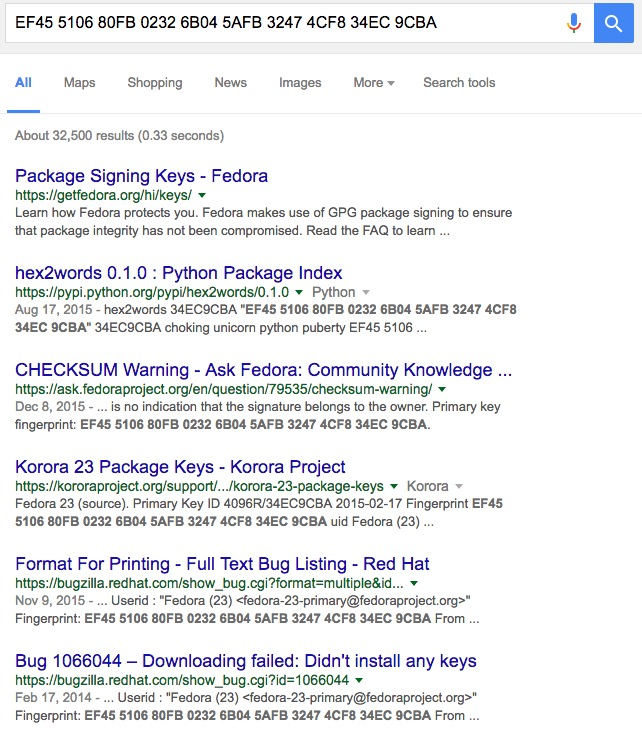
\includegraphics[width=\linewidth]{./images/google_key.jpg}
    \caption{Google search results for Fedora 23's public key fingerprint}
\label{fedora_google}
\end{figure}


\subsection{Patience and ``Soft'' Risk Mitigation}

Many users install a new operating system immediately after it is released. We recommend
that a security-conscious individual download the image, signed checksum and keys immediately
and then wait for some period of time. If the image, signature or keys were replaced by an
attack before release, then the time when it is most likely to be noticed is when people
are looking around the new system for new features, bugs and other anomalies. After waiting,
the user can download everything again and ensure that all the items match.

\section{Automation}

Initially, we planned to write scripts to automate our recommendations of best practices
for several distributions. However, over the course of our research, we decided that this
would likely have a negative impact on security. One reason for this is the fragility of
such a script. For example, to automate downloading files from several mirrors for Fedora
Linux, we would either have to hard-code the mirror links or scrape the HTML from the
official mirrors list. Hard-coded links would be unreliable and eventually break. Scraping
the HTML would break when the format of the mirrors list changed. 
Either of these options would be inferior to a person applying
common sense and reasoning to the same process. Once we had the correct server link, we would
also have to append a hard-coded file path that contains the release version number. The version
number would change at the next version release and the file path could as well. Another
problem is that analyzing Google
search results is fairly easy for a person but a script would be unreliable at best.
We posit that downloading an image for a new operating system is an infrequent and 
important enough task that the person wishing to do so should devote their full attention
to the task.

% An example of a floating figure using the graphicx package.
% Note that \label must occur AFTER (or within) \caption.
% For figures, \caption should occur after the \includegraphics.
% Note that IEEEtran v1.7 and later has special internal code that
% is designed to preserve the operation of \label within \caption
% even when the captionsoff option is in effect. However, because
% of issues like this, it may be the safest practice to put all your
% \label just after \caption rather than within \caption{}.
%
% Reminder: the "draftcls" or "draftclsnofoot", not "draft", class
% option should be used if it is desired that the figures are to be
% displayed while in draft mode.
%
%\begin{figure}[!t]
%\centering
%\includegraphics[width=2.5in]{myfigure}
% where an .eps filename suffix will be assumed under latex, 
% and a .pdf suffix will be assumed for pdflatex; or what has been declared
% via \DeclareGraphicsExtensions.
%\caption{Simulation results for the network.}
%\label{fig_sim}
%\end{figure}

% Note that the IEEE typically puts floats only at the top, even when this
% results in a large percentage of a column being occupied by floats.


% An example of a double column floating figure using two subfigures.
% (The subfig.sty package must be loaded for this to work.)
% The subfigure \label commands are set within each subfloat command,
% and the \label for the overall figure must come after \caption.
% \hfil is used as a separator to get equal spacing.
% Watch out that the combined width of all the subfigures on a 
% line do not exceed the text width or a line break will occur.
%
%\begin{figure*}[!t]
%\centering
%\subfloat[Case I]{\includegraphics[width=2.5in]{box}%
%\label{fig_first_case}}
%\hfil
%\subfloat[Case II]{\includegraphics[width=2.5in]{box}%
%\label{fig_second_case}}
%\caption{Simulation results for the network.}
%\label{fig_sim}
%\end{figure*}
%
% Note that often IEEE papers with subfigures do not employ subfigure
% captions (using the optional argument to \subfloat[]), but instead will
% reference/describe all of them (a), (b), etc., within the main caption.
% Be aware that for subfig.sty to generate the (a), (b), etc., subfigure
% labels, the optional argument to \subfloat must be present. If a
% subcaption is not desired, just leave its contents blank,
% e.g., \subfloat[].


% An example of a floating table. Note that, for IEEE style tables, the
% \caption command should come BEFORE the table and, given that table
% captions serve much like titles, are usually capitalized except for words
% such as a, an, and, as, at, but, by, for, in, nor, of, on, or, the, to
% and up, which are usually not capitalized unless they are the first or
% last word of the caption. Table text will default to \footnotesize as
% the IEEE normally uses this smaller font for tables.
% The \label must come after \caption as always.
%
%\begin{table}[!t]
%% increase table row spacing, adjust to taste
%\renewcommand{\arraystretch}{1.3}
% if using array.sty, it might be a good idea to tweak the value of
% \extrarowheight as needed to properly center the text within the cells
%\caption{An Example of a Table}
%\label{table_example}
%\centering
%% Some packages, such as MDW tools, offer better commands for making tables
%% than the plain LaTeX2e tabular which is used here.
%\begin{tabular}{|c||c|}
%\hline
%One & Two\\
%\hline
%Three & Four\\
%\hline
%\end{tabular}
%\end{table}


% Note that the IEEE does not put floats in the very first column
% - or typically anywhere on the first page for that matter. Also,
% in-text middle ("here") positioning is typically not used, but it
% is allowed and encouraged for Computer Society conferences (but
% not Computer Society journals). Most IEEE journals/conferences use
% top floats exclusively. 
% Note that, LaTeX2e, unlike IEEE journals/conferences, places
% footnotes above bottom floats. This can be corrected via the
% \fnbelowfloat command of the stfloats package.




\section{Conclusion}

Image and source distribution creates an attack surface for any
operating system. Some maintainers of open source distributions
appear to be neglecting this issue and, in the process, exposing
their users to potential harm. Other groups are paying attention
and following best practices, and a few are even trying to push
the field forward. We found ways that consumers can proactively
protect themselves and identify distributions with signs of
bad practices. Risk can be seriously mitigated on an individual
level with some caution and patience.

% conference papers do not normally have an appendix


% use section* for acknowledgment
% trigger a \newpage just before the given reference
% number - used to balance the columns on the last page
% adjust value as needed - may need to be readjusted if
% the document is modified later
%\IEEEtriggeratref{8}
% The "triggered" command can be changed if desired:
%\IEEEtriggercmd{\enlargethispage{-5in}}

% references section

% can use a bibliography generated by BibTeX as a .bbl file
% BibTeX documentation can be easily obtained at:
% http://mirror.ctan.org/biblio/bibtex/contrib/doc/
% The IEEEtran BibTeX style support page is at:
% http://www.michaelshell.org/tex/ieeetran/bibtex/
\bibliography{references.bib}
\bibliographystyle{IEEEtran}
% argument is your BibTeX string definitions and bibliography database(s)
%\bibliography{IEEEabrv,../bib/paper}
%
% <OR> manually copy in the resultant .bbl file
% set second argument of \begin to the number of references
% (used to reserve space for the reference number labels box)
%\newcommand{\bibspace}[1] {\hskip 0.5em}
%\begin{thebibliography}{1}
%\end{thebibliography}

% that's all folks
\end{document}
